\section{Code Structure}

The three core classes, the \texttt{Astrocyte}, \texttt{SMCEC} and \texttt{WallMechanics}, correspond to the components of the NVU model, namely the astrocyte model, the SMC and EC model, and the mechanical contraction cell model. For a given model component, all fluxes and ODEs are grouped together in the code of the corresponding class. The \texttt{NVU} class uses the three core component classes to collect the state variable and derivatives values and pass them to the \texttt{ode15s} solver for stiff problems. All classes in OO-NVU code are subclasses of the MATLAB's \texttt{handle} class which makes them appear as reference object to avoid unnecessary object duplication on assignment. Figure~\ref{fig:OO-Code-Structure} shows the public interfaces for all OO-NVU classes.

\todo[inline]{For a proper OO development and complexity management in the future the Astrocyte, SMCEC and the WallMechanics classes should have a common superclass with the shared interface (at least) and functionality. --Kon}

The following features apply to the \texttt{Astrocyte}, \texttt{SMCEC} and \texttt{WallMechanics} classes:

\begin{enumerate}
	\item The core classes rely on the class constructors to initialise the parameters with the help of the class-specific function \text{parse\_inputs(varangin)}. The constructors also initialise the variable indices, initial conditions and the output indices.
	
	\item In every core class the \texttt{rhs} method contains the algebraic and state variables, as well as the corresponding equations.
	
	\item The \texttt{shared(self, \~{}, u)} method, where present, provides the access to the shared algebraic or state variables used as input variables in the other model components where appropriate.
\end{enumerate}

\begin{figure}[htb!]
	\centering
	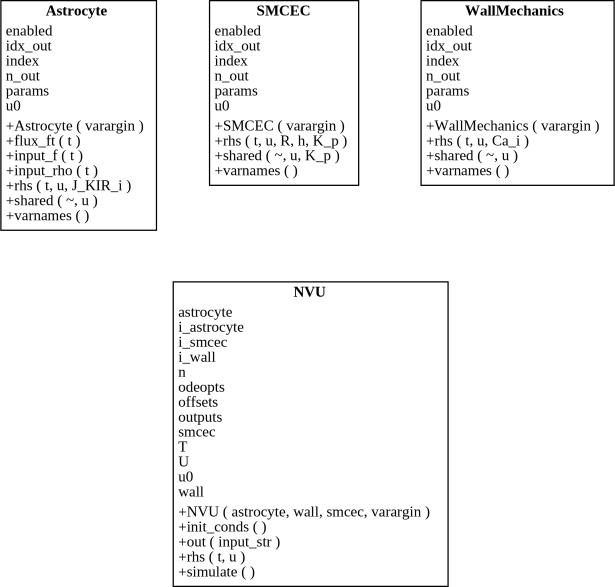
\includegraphics[width=0.7\linewidth]{figures/OO-Code-Structure}
	\caption[OO NVU Classes]{UML class diagram for the OO NVU code.}
	\label{fig:OO-Code-Structure}
\end{figure}

The code in the file \texttt{nvu\_script.m} provides a number of use-cases for running the NVU model. The code Listing~\ref{lst:NVU-Model-Init} shows an example of setting the options for the ODE solver \texttt{ode15s} specifying the \texttt{odeopts} parameter, however the code works well with default tolerances. The \texttt{simulate()} method of the \texttt{NVU} class start the simulation.

\begin{lstlisting}[language=Matlab,caption={Initialisation of the NVU model components.},label={lst:NVU-Model-Init},frameround=tttt,belowcaptionskip=10pt]
odeopts = odeset('RelTol', 1e-03, 'AbsTol', 1e-03, 'MaxStep', 1, 'Vectorized', 1);

nv = NVU(Astrocyte(), ...
WallMechanics(), ...
SMCEC('J_PLC', 0.18), ...
'odeopts', odeopts);

nv.simulate()
\end{lstlisting}


